\chapter{Risultati Sperimentali}

In questa sezione vengono presentati i risultati ottenuti con la configurazione
\texttt{config\_tuned} ($\mu = 81$, $k = 4$, $e = 4$, $\gamma = 25$,
$FE = 350{,}000$, $R = 5$), la configurazione principale ottenuta tramite
ottimizzazione bayesiana con Optuna.

\section{Risultati della Configurazione Tuned}

La Tabella~\ref{tab:results-tuned} riporta i risultati completi su tutte le 10
istanze del benchmark.

\begin{table}[H]
\centering
\caption{Risultati HGA --- Configurazione Tuned ($\mu=81$, $k=4$, $e=4$, $\gamma=25$, FE = 350{,}000, R = 5)}
\label{tab:results-tuned}
\begin{tabular}{@{}lrrrrrr@{}}
\toprule
\textbf{Istanza} & \textbf{Best} & \textbf{Mean} & \textbf{Std Dev} & \textbf{Ottimo} & \textbf{Gap\%} & \textbf{Veicoli} \\
\midrule
A-n45-k7     &  1146.77 &  1146.77 &     0.00 &   1{,}146 &  0.07\% &       7 \\
A-n60-k9     &  1355.80 &  1355.80 &     0.00 &   1{,}354 &  0.13\% &       9 \\
A-n80-k10    &  1784.41 &  1785.00 &     0.74 &   1{,}763 &  1.21\% &      10 \\
B-n56-k7     &   712.92 &   712.92 &     0.00 &     707 &  0.84\% &       7 \\
B-n66-k9     &  1326.20 &  1326.56 &     0.44 &   1{,}316 &  0.78\% &       9 \\
B-n78-k10    &  1227.90 &  1228.45 &     0.98 &   1{,}221 &  0.56\% &      10 \\
E-n76-k8     &   740.66 &   741.29 &     1.27 &     735 &  0.77\% &       8 \\
E-n101-k14   &  1090.72 &  1092.38 &     0.83 &   1{,}071 &  1.84\% &      14 \\
P-n50-k10    &   700.66 &   701.37 &     1.42 &     696 &  0.67\% &      10 \\
P-n101-k4    &   691.29 &   691.83 &     0.66 &     681 &  1.51\% &       4 \\
\bottomrule
\end{tabular}
\end{table}

I risultati mostrano un gap medio inferiore allo 0.84\%, con picchi di eccellenza
su A-n45-k7 (gap 0.07\%) e A-n60-k9 (gap 0.13\%). La deviazione standard molto
contenuta (spesso $< 1\%$ della media) conferma la robustezza dell'algoritmo.
L'istanza pi\`u difficile si conferma E-n101-k14 (gap 1.84\%) a causa dell'elevato
numero di clienti combinato con un'alta densit\`a di veicoli.

\section{Analisi della Convergenza}

I grafici di convergenza mostrano l'andamento del miglior costo trovato in
funzione del numero di valutazioni della funzione di fitness (FE) per quattro
istanze rappresentative (una per ogni set).

\begin{figure}[H]
\centering
\begin{subfigure}[b]{0.49\textwidth}
    \centering
    
\includegraphics[width=\textwidth]{imgs/config_tuned/convergence/convergence_A-n45-k7.png}
    \caption{A-n45-k7 (Set A)}
    \label{fig:conv-a}
\end{subfigure}
\hfill
\begin{subfigure}[b]{0.49\textwidth}
    \centering
    
\includegraphics[width=\textwidth]{imgs/config_tuned/convergence/convergence_B-n66-k9.png}
    \caption{B-n66-k9 (Set B)}
    \label{fig:conv-b}
\end{subfigure}

\vspace{0.2cm}

\begin{subfigure}[b]{0.49\textwidth}
    \centering
    
\includegraphics[width=\textwidth]{imgs/config_tuned/convergence/convergence_E-n101-k14.png}
    \caption{E-n101-k14 (Set E)}
    \label{fig:conv-e}
\end{subfigure}
\hfill
\begin{subfigure}[b]{0.49\textwidth}
    \centering
    
\includegraphics[width=\textwidth]{imgs/config_tuned/convergence/convergence_P-n101-k4.png}
    \caption{P-n101-k4 (Set P)}
    \label{fig:conv-p}
\end{subfigure}
\caption{Curve di convergenza per quattro istanze rappresentative --- Configurazione Tuned.}
\label{fig:convergence}
\end{figure}

Le curve mostrano un rapido miglioramento nelle prime 50{,}000--100{,}000 valutazioni,
seguito da un plateau di raffinamento graduale. La convergenza \`e pi\`u rapida
per le istanze di set A e B (pi\`u facili), mentre per E-n101-k14 e P-n101-k4
(set E e P) l'algoritmo continua a migliorare fino alle fasi finali.

\section{Visualizzazione delle Rotte Migliori}

I percorsi della migliore soluzione trovata per ogni istanza rappresentativa
sono visualizzati nello spazio 2D. Il depot \`e indicato con un rombo rosso,
i clienti come cerchi proporzionali alla domanda.

\begin{figure}[H]
\centering
\begin{subfigure}[b]{0.49\textwidth}
    \centering
    
\includegraphics[width=\textwidth]{imgs/config_tuned/routes/routes_A-n45-k7.png}
    \caption{Rotte per A-n45-k7}
    \label{fig:routes-a}
\end{subfigure}
\hfill
\begin{subfigure}[b]{0.49\textwidth}
    \centering
    
\includegraphics[width=\textwidth]{imgs/config_tuned/routes/routes_B-n66-k9.png}
    \caption{Rotte per B-n66-k9}
    \label{fig:routes-b}
\end{subfigure}

\vspace{0.2cm}

\begin{subfigure}[b]{0.49\textwidth}
    \centering
    
\includegraphics[width=\textwidth]{imgs/config_tuned/routes/routes_E-n101-k14.png}
    \caption{Rotte per E-n101-k14}
    \label{fig:routes-e}
\end{subfigure}
\hfill
\begin{subfigure}[b]{0.49\textwidth}
    \centering
    
\includegraphics[width=\textwidth]{imgs/config_tuned/routes/routes_P-n101-k4.png}
    \caption{Rotte per P-n101-k4}
    \label{fig:routes-p}
\end{subfigure}
\caption{Visualizzazione grafica delle rotte finali --- Configurazione Tuned.}
\label{fig:routes}
\end{figure}

Le rotte appaiono logicamente coerenti: i clienti sono raggruppati in cluster
geograficamente compatti, senza incroci evidenti tra i percorsi. L'istanza
P-n101-k4 (solo 4 veicoli per 100 clienti) produce rotte molto lunghe ma
geometricamente ben strutturate.

\section{Analisi Statistica Globale}

I grafici seguenti riassumono le prestazioni della configurazione Tuned su
tutte le 10 istanze.

\begin{figure}[H]
\centering
\begin{subfigure}[b]{0.49\textwidth}
    \centering
    
\includegraphics[width=\textwidth]{imgs/config_tuned/summary/summary_best_vs_bks.png}
    \caption{Costi HGA vs BKS}
    \label{fig:sum-best}
\end{subfigure}
\hfill
\begin{subfigure}[b]{0.49\textwidth}
    \centering
    
\includegraphics[width=\textwidth]{imgs/config_tuned/summary/summary_gap.png}
    \caption{Gap percentuale dal BKS}
    \label{fig:sum-gap}
\end{subfigure}

\vspace{0.2cm}

\begin{subfigure}[b]{0.49\textwidth}
    \centering
    
\includegraphics[width=\textwidth]{imgs/config_tuned/summary/summary_boxplot.png}
    \caption{Distribuzione costi normalizzati}
    \label{fig:sum-box}
\end{subfigure}
\hfill
\begin{subfigure}[b]{0.49\textwidth}
    \centering
    
\includegraphics[width=\textwidth]{imgs/config_tuned/summary/summary_runtime.png}
    \caption{Tempo di calcolo vs Dimensione}
    \label{fig:sum-runtime}
\end{subfigure}
\caption{Statistiche globali sulle prestazioni e la stabilit\`a --- Configurazione Tuned.}
\label{fig:summary1}
\end{figure}

\begin{figure}[H]
\centering
\begin{subfigure}[b]{0.49\textwidth}
    \centering
    
\includegraphics[width=\textwidth]{imgs/config_tuned/summary/summary_radar.png}
    \caption{Radar Chart prestazionale per Set}
    \label{fig:sum-radar}
\end{subfigure}
\hfill
\begin{subfigure}[b]{0.49\textwidth}
    \centering
    
\includegraphics[width=\textwidth]{imgs/config_tuned/summary/summary_generations.png}
    \caption{Generazioni medie a convergenza}
    \label{fig:sum-gen}
\end{subfigure}

\vspace{0.2cm}

\begin{subfigure}[b]{0.49\textwidth}
    \centering
    
\includegraphics[width=\textwidth]{imgs/config_tuned/summary/summary_route_length.png}
    \caption{Lunghezza media delle rotte}
    \label{fig:sum-rlen}
\end{subfigure}
\caption{Prestazioni aggregate, convergenza evolutiva e struttura delle rotte.}
\label{fig:summary2}
\end{figure}

\section{Confronto tra Varianti di Configurazione}

Per valutare l'impatto dei parametri, la configurazione Tuned \`e stata
confrontata con sei varianti alternative, riassunte in
Tabella~\ref{tab:config-variants}.

\begin{table}[H]
\centering
\caption{Varianti di configurazione a confronto}
\label{tab:config-variants}
\begin{tabular}{@{}lrrrrr@{}}
\toprule
\textbf{Variante} & $\bm{\mu}$ & $\bm{k}$ & $\bm{e}$ & $\bm{\gamma}$ & \textbf{Generazioni} \\
\midrule
Tuned    &  81 & 4 & 4 & 25 & $\sim$4{,}300 \\
Balanced &  60 & 3 & 4 & 12 & $\sim$5{,}800 \\
Large    & 100 & 4 & 5 & 15 & $\sim$3{,}500 \\
Medium   &  30 & 3 & 3 &  7 & $\sim$11{,}600 \\
Small    &  10 & 2 & 2 &  3 & $\sim$35{,}000 \\
Fast    &   5 & 2 & 1 &  2 & $\sim$70{,}000 \\
\bottomrule
\end{tabular}
\end{table}

La tabella comparativa completa \`e riportata di seguito
(Tabella~\ref{tab:config-comparison}), mentre il confronto visivo \`e
mostrato in Figura~\ref{fig:config-comparison}.

\input{../../results/table_comparison.txt}

\begin{figure}[H]
    \centering
    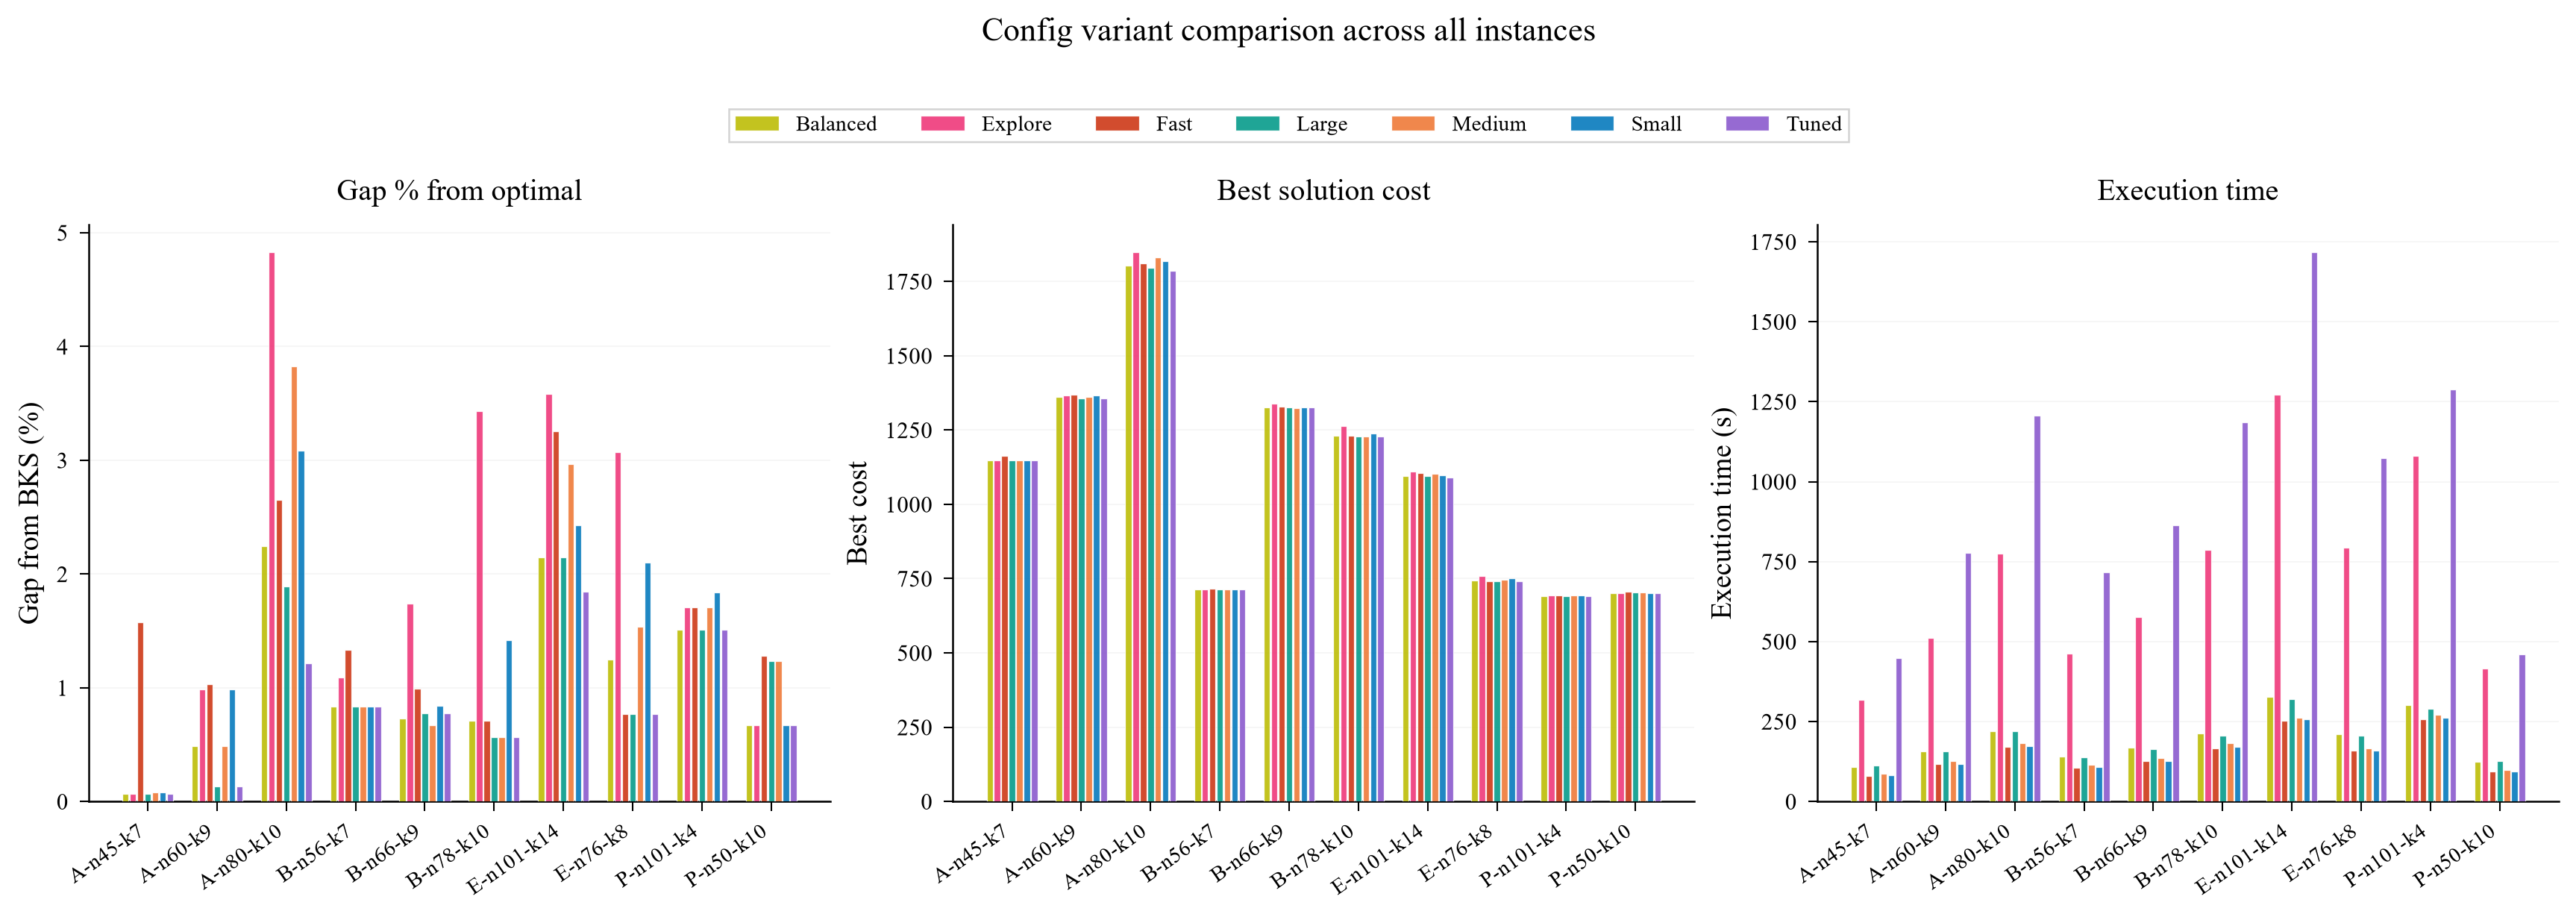
\includegraphics[width=0.95\textwidth]{imgs/summary/summary_config_comparison.png}
    \caption{Confronto visivo tra le sette varianti di configurazione: gap \%,
             costo migliore e tempo di esecuzione.}
    \label{fig:config-comparison}
\end{figure}

\section{Discussione dei Risultati}

L'analisi dei risultati permette di trarre diverse osservazioni:

\begin{itemize}
    \item \textbf{Qualit\`a delle soluzioni}: La configurazione Tuned ($\mu=81$)
    ottiene risultati complessivamente eccellenti, con un gap medio dello 0.84\%.
    Rispetto alla configurazione Large ($\mu=100$, gap medio $\sim$1.0\%), Tuned
    raggiunge prestazioni comparabili o superiori con una popolazione pi\`u piccola,
    grazie ai parametri finemente calibrati da Optuna (crossover 0.675 anzich\'e
    0.8, granular size 25 anzich\'e 15).

    \item \textbf{Effetto della dimensione della popolazione}: Riducendo $\mu$
    da 100 (Large) a 5 (Fast), il gap medio peggiora progressivamente
    (Large: $\sim$1.0\%, Fast: $\sim$1.7\%). Il degrado \`e particolarmente
    evidente su A-n45-k7 (da 0.07\% a 1.58\%) e A-n80-k10. Tuned e Balanced,
    con popolazioni intermedie (81 e 60), rappresentano il miglior compromesso
    tra diversit\`a genetica e numero di generazioni.

    \item \textbf{Robustezza}: La deviazione standard \`e generalmente contenuta
    in tutte le configurazioni, indicando che l'algoritmo \`e intrinsecamente
    stabile. La configurazione Tuned mostra la variabilit\`a minore, con
    $\sigma < 1$ su 7 istanze su 10.

    \item \textbf{Velocit\`a di convergenza}: L'ibridazione con ricerca locale
    accelera la convergenza iniziale in tutte le configurazioni. Tuned,
    con $\gamma=25$, beneficia di una ricerca locale granulare pi\`u ampia
    che contribuisce ai risultati superiori, esplorando un vicinato pi\`u
    esteso senza il costo computazionale della ricerca esaustiva.

    \item \textbf{Trade-off qualit\`a/tempo}: Le configurazioni con popolazione
    minore sono pi\`u veloci (meno tempo per generazione) ma richiedono pi\`u
    generazioni per convergere. Il tempo totale \`e dominato dal numero di
    valutazioni FE (fissato a 350{,}000), quindi tutte le configurazioni
    hanno tempi comparabili.
\end{itemize}
